\documentclass{beamer}
\mode<presentation>
\usepackage{amsmath}
\usepackage{amssymb}
%\usepackage{advdate}
\usepackage{adjustbox}
\usepackage{subcaption}
\usepackage{enumitem}
\usepackage{multicol}
\usepackage{mathtools}
\usepackage{listings}
\usepackage{float}
\usepackage{graphicx}
\usepackage{url}
\def\UrlBreaks{\do\/\do-}
\usetheme{Boadilla}
\usecolortheme{lily}
\setbeamertemplate{footline}
{
  \leavevmode%
  \hbox{%
  \begin{beamercolorbox}[wd=\paperwidth,ht=2.25ex,dp=1ex,right]{author in head/foot}%
    \insertframenumber{} / \inserttotalframenumber\hspace*{2ex} 
  \end{beamercolorbox}}%
  \vskip0pt%
}
\setbeamertemplate{navigation symbols}{}

\providecommand{\nCr}[2]{\,^{#1}C_{#2}} % nCr
\providecommand{\nPr}[2]{\,^{#1}P_{#2}} % nPr
\providecommand{\mbf}{\mathbf}
\providecommand{\pr}[1]{\ensuremath{\Pr\left(#1\right)}}
\providecommand{\qfunc}[1]{\ensuremath{Q\left(#1\right)}}
\providecommand{\sbrak}[1]{\ensuremath{{}\left[#1\right]}}
\providecommand{\lsbrak}[1]{\ensuremath{{}\left[#1\right.}}
\providecommand{\rsbrak}[1]{\ensuremath{{}\left.#1\right]}}
\providecommand{\brak}[1]{\ensuremath{\left(#1\right)}}
\providecommand{\lbrak}[1]{\ensuremath{\left(#1\right.}}
\providecommand{\rbrak}[1]{\ensuremath{\left.#1\right)}}
\providecommand{\cbrak}[1]{\ensuremath{\left\{#1\right\}}}
\providecommand{\lcbrak}[1]{\ensuremath{\left\{#1\right.}}
\providecommand{\rcbrak}[1]{\ensuremath{\left.#1\right\}}}
\theoremstyle{remark}
\newtheorem{rem}{Remark}
\newcommand{\sgn}{\mathop{\mathrm{sgn}}}
\providecommand{\abs}[1]{\left\vert#1\right\vert}
\providecommand{\res}[1]{\Res\displaylimits_{#1}} 
\providecommand{\norm}[1]{\lVert#1\rVert}
\providecommand{\mtx}[1]{\mathbf{#1}}
\providecommand{\mean}[1]{E\left[ #1 \right]}
\providecommand{\fourier}{\overset{\mathcal{F}}{ \rightleftharpoons}}
%\providecommand{\hilbert}{\overset{\mathcal{H}}{ \rightleftharpoons}}
\providecommand{\system}{\overset{\mathcal{H}}{ \longleftrightarrow}}
	%\newcommand{\solution}[2]{\textbf{Solution:}{#1}}
%\newcommand{\solution}{\noindent \textbf{Solution: }}
\providecommand{\dec}[2]{\ensuremath{\overset{#1}{\underset{#2}{\gtrless}}}}
\newcommand{\myvec}[1]{\ensuremath{\begin{pmatrix}#1\end{pmatrix}}}
\let\vec\mathbf

\lstset{
language=C,
frame=single, 
breaklines=true,
columns=fullflexible
}

\numberwithin{equation}{section}

\title{Presentation - Matgeo}
\author{Aryansingh Sonaye \\
AI25BTECH11032 \\
EE1030 - Matrix Theory}

\date{\today} 
\begin{document}

\begin{frame}
\titlepage
\end{frame}

\section{Problem}
\begin{frame}
\frametitle{Problem Statement}
\section*{Problem 8.3.12}
Find the equation of the set of all points the sum of whose distances 
from the points $\myvec{3\\0}$ and $\myvec{9\\0}$ is $12$.


\end{frame}

\section{Solution}
\subsection{Description of Variables used}
\begin{frame}
\frametitle{Description of Variables used}
\begin{table}[H]
\centering
\begin{tabular}{|c|c|}
\hline
Variable & Value \\
\hline
$\vec F_1$ & $\myvec{3\\0}$ \\
\hline
$\vec F_2$ & $\myvec{9\\0}$ \\
\hline
$2a$ & $12$ \\
\hline
\end{tabular}
\caption{} \label{}
\end{table}


\end{frame}

\subsection{Theoretical Solution }
\begin{frame}
\frametitle{Theoretical Solution}
\textbf{Step 1: Center and axis data}
\begin{align}
\vec c &= \frac{\vec F_1+\vec F_2}{2}=\myvec{6\\0}, &
\vec v &= \frac{\vec F_2-\vec F_1}{\|\vec F_2-\vec F_1\|}=\myvec{1\\0}, &
c_f &= \frac{\|\vec F_2-\vec F_1\|}{2}=3, &
a &= 6.
\end{align}
Shift to the midpoint frame: $\vec y:=\vec x-\vec c$.

\textbf{Step 2: Start from the sum-of-distances definition}
\begin{align}
\|\vec y-c_f\vec v\|+\|\vec y+c_f\vec v\|=2a.
\end{align}

\textbf{Step 3: Eliminate square roots (squaring twice)}
Let $r_\pm:=\|\vec y\pm c_f\vec v\|$. From (3.2), $r_++r_-=2a$.
\begin{align}
r_+r_- &= 2a^2-\|\vec y\|^2-c_f^2, \\
r_+-r_- &= \frac{2c_f}{a}\,\vec v^\top\vec y
\;\Rightarrow\;
r_+r_- = a^2-\frac{c_f^2}{a^2}(\vec v^\top\vec y)^2.
\end{align}

\end{frame}

\begin{frame}
\frametitle{Theoretical Solution}
Equating the two expressions for $r_+r_-$ yields
\begin{align}
\|\vec y\|^2-\frac{c_f^2}{a^2}(\vec v^\top\vec y)^2 = a^2-c_f^2 \;=:\; b^2.
\end{align}

\textbf{Step 4: Principal directions and the matrix $D$}

Choose an orthonormal basis of principal directions:
\begin{align}
\vec p_1 &= \vec v, \qquad \vec p_2 \perp \vec p_1, \qquad
P:=\myvec{\vec p_1 & \vec p_2} \;\;\text{(orthonormal)}.
\end{align}
Decompose $\vec y$ as $\vec y = \alpha\,\vec p_1 + \beta\,\vec p_2$, where
$\alpha=\vec p_1^\top\vec y=\vec v^\top\vec y$ and $\beta=\vec p_2^\top\vec y$.
Then $\|\vec y\|^2=\alpha^2+\beta^2$. Substituting into (5) gives
\begin{align}
\frac{\alpha^2}{a^2}+\frac{\beta^2}{b^2}=1.
\end{align}
In matrix form this is

\end{frame}

\begin{frame}
\frametitle{Theoretical Solution}
\begin{align}
\vec y^\top \Big(P\,\mathrm{diag}\!\big(\tfrac{1}{a^2},\tfrac{1}{b^2}\big)\,P^\top\Big)\vec y = 1.
\end{align}
Hence define
\begin{align}
D := P\,\mathrm{diag}\!\Big(\tfrac{1}{a^2},\tfrac{1}{b^2}\Big)\,P^\top,
\qquad\text{so that}\qquad
(\vec x-\vec c)^\top D\,(\vec x-\vec c)=1. 
\end{align}

\textbf{Step 5: Specialization to this data}

Here $\vec p_1=\myvec{1\\0},\ \vec p_2=\myvec{0\\1}$, so $P=I$ and
\begin{align}
b^2 &= a^2-c_f^2 = 36-9=27, \\
D &= \mathrm{diag}\!\Big(\tfrac{1}{a^2},\tfrac{1}{b^2}\Big)
= \myvec{\tfrac{1}{36}&0\\[2pt]0&\tfrac{1}{27}}.
\end{align}

\end{frame}

\begin{frame}
\frametitle{Theoretical Solution}
Therefore the \textbf{centered matrix equation of the locus} is exactly (9) with
\begin{align}
\boxed{\;(\vec x-\myvec{6\\0})^\top
\myvec{\tfrac{1}{36}&0\\[2pt]0&\tfrac{1}{27}}
(\vec x-\myvec{6\\0})=1\;}
\end{align}

\textbf{Step 6: General quadratic (matrix) form}

Expanding (9) gives $\vec x^\top V\vec x+2\vec u^\top\vec x+f=0$ with
\begin{align}
V &= D, &
\vec u &= -V\vec c, &
f &= \vec c^\top V\vec c - 1.
\end{align}
Numerically,
\begin{align}
\boxed{\;
V=\myvec{\tfrac{1}{36}&0\\[2pt]0&\tfrac{1}{27}},\quad
\vec u=\myvec{-\tfrac{1}{6}\\[2pt]0},\quad
f=0\; }.
\end{align}

\end{frame}


\subsection{Plot}
\begin{frame}
    \frametitle{Plot}
\begin{figure}[H]
   \centering
   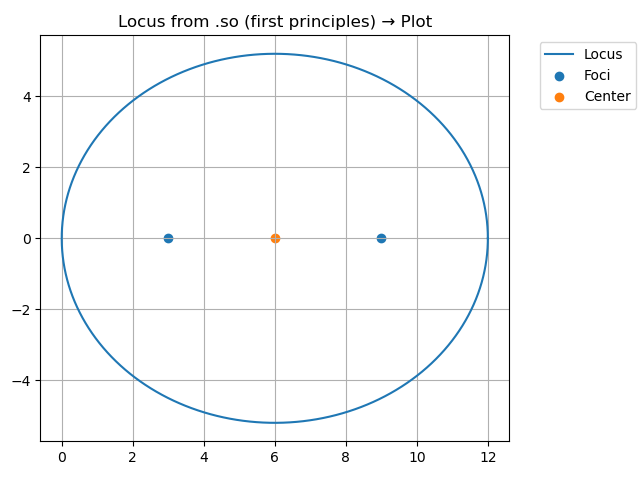
\includegraphics[width=0.8\columnwidth]{figs/ellipse.png}
   \caption{}
   \label{}
   \end{figure}
\end{frame}

\begin{frame}[fragile]
    \frametitle{Code - C}
    \begin{lstlisting}
#include <math.h>

void ellipse_params(const double *F1, const double *F2, double sum,
                    double *V, double *u, double *f,
                    double *c, double *a_out, double *b_out)
{
    // center
    c[0] = 0.5 * (F1[0] + F2[0]);
    c[1] = 0.5 * (F1[1] + F2[1]);

    // a, cf, b
    double a = 0.5 * sum;
    double dx = F2[0] - F1[0];
    double dy = F2[1] - F1[1];
    double cf = 0.5 * sqrt(dx*dx + dy*dy);
    double b2 = a*a - cf*cf;
    double b  = sqrt(b2);



    \end{lstlisting}
    \end{frame}

    \begin{frame}[fragile]
    \frametitle{Code - C}
    \begin{lstlisting}
    if (a_out) *a_out = a;
    if (b_out) *b_out = b;

    // V = diag(1/a^2, 1/b^2)
    V[0] = 1.0/(a*a); V[1] = 0.0;
    V[2] = 0.0;       V[3] = 1.0/(b*b);

    // u = -V c
    u[0] = -(V[0]*c[0] + V[1]*c[1]);
    u[1] = -(V[2]*c[0] + V[3]*c[1]);

    // f = c^T V c - 1
    *f = c[0]*(V[0]*c[0] + V[1]*c[1]) + c[1]*(V[2]*c[0] + V[3]*c[1]) - 1.0;
}

    \end{lstlisting}
    \end{frame}

\begin{frame}[fragile]
    \frametitle{Code - Python(with shared C code)}
    The code to obtain the required plot is
    \begin{lstlisting}
import ctypes as ct
import numpy as np
import matplotlib.pyplot as plt

# Load the shared library
# On macOS, use: lib = ct.CDLL("./libellipse_simple.dylib")
lib = ct.CDLL("./libellipse_simple.so")

# Set function signature
lib.ellipse_params.argtypes = [
    ct.POINTER(ct.c_double),  # F1
    ct.POINTER(ct.c_double),  # F2
    ct.c_double,              # sum (2a)
    ct.POINTER(ct.c_double),  # V (len 4, row-major)
    ct.POINTER(ct.c_double),  # u (len 2)
    ct.POINTER(ct.c_double),  # f (scalar)



\end{lstlisting}
\end{frame}
\begin{frame}[fragile]
\frametitle{Code - Python(with shared C code)}
\begin{lstlisting}
    ct.POINTER(ct.c_double),  # c (len 2)
    ct.POINTER(ct.c_double),  # a_out (scalar)
    ct.POINTER(ct.c_double),  # b_out (scalar)
]
lib.ellipse_params.restype = None
# Inputs (your problem)
F1 = np.array([3.0, 0.0], dtype=np.float64)
F2 = np.array([9.0, 0.0], dtype=np.float64)
sum_dist = 12.0

# Outputs
V = np.zeros(4, dtype=np.float64)
u = np.zeros(2, dtype=np.float64)
f = np.zeros(1, dtype=np.float64)
c = np.zeros(2, dtype=np.float64)
a = np.zeros(1, dtype=np.float64)
b = np.zeros(1, dtype=np.float64)


\end{lstlisting}
\end{frame}

\begin{frame}[fragile]
\frametitle{Code - Python(with shared C code)}
\begin{lstlisting}
# Call the C function
lib.ellipse_params(
    F1.ctypes.data_as(ct.POINTER(ct.c_double)),
    F2.ctypes.data_as(ct.POINTER(ct.c_double)),
    ct.c_double(sum_dist),
    V.ctypes.data_as(ct.POINTER(ct.c_double)),
    u.ctypes.data_as(ct.POINTER(ct.c_double)),
    f.ctypes.data_as(ct.POINTER(ct.c_double)),
    c.ctypes.data_as(ct.POINTER(ct.c_double)),
    a.ctypes.data_as(ct.POINTER(ct.c_double)),
    b.ctypes.data_as(ct.POINTER(ct.c_double)),
)
print("V =\n", V.reshape(2,2))
print("u =", u)
print("f =", f[0])
print("center c =", c)
print("a, b =", a[0], b[0])


\end{lstlisting}
\end{frame}

\begin{frame}[fragile]
\frametitle{Code - Python(with shared C code)}
\begin{lstlisting}
# Parametric plot (simple & direct)
t = np.linspace(0, 2*np.pi, 600)
x = c[0] + a[0]*np.cos(t)
y = c[1] + b[0]*np.sin(t)

plt.plot(x, y, label="Locus")
plt.scatter([F1[0], F2[0]], [F1[1], F2[1]], label="Foci")
plt.scatter([c[0]], [c[1]], label="Center")
plt.gca().set_aspect("equal", adjustable="box")
plt.grid(True)
plt.legend(loc="upper left", bbox_to_anchor=(1.05, 1.0))
plt.title("Locus from .so (first principles) => Plot")
plt.tight_layout()
plt.savefig("ellipse.png")
plt.show()



\end{lstlisting}
\end{frame}



\begin{frame}[fragile]
\frametitle{Code - Python only}
\begin{lstlisting}
import numpy as np
import matplotlib.pyplot as plt

def ellipse_params_from_foci(F1, F2, s):
    F1 = np.asarray(F1, dtype=float)
    F2 = np.asarray(F2, dtype=float)
    c  = 0.5 * (F1 + F2)
    a  = 0.5 * s
    d  = np.linalg.norm(F2 - F1)
    cf = 0.5 * d
    b2 = a*a - cf*cf
    if b2 <= 0:
        raise ValueError("Inputs do not define a real ellipse (b^2 <= 0).")
    b  = np.sqrt(b2)



\end{lstlisting}
\end{frame}

\begin{frame}[fragile]
\frametitle{Code - Python only}
\begin{lstlisting}
    # Axis-aligned case (since foci are on a line here)
    V = np.diag([1.0/(a*a), 1.0/(b*b)])
    u = -V @ c
    f = float(c @ (V @ c) - 1.0)
    return V, u, f, c, a, b

def plot_ellipse(c, a, b, F1=None, F2=None, n=600):
    t = np.linspace(0, 2*np.pi, n)
    x = c[0] + a*np.cos(t)
    y = c[1] + b*np.sin(t)

    plt.plot(x, y, label="Locus")
    if F1 is not None and F2 is not None:
        plt.scatter([F1[0], F2[0]], [F1[1], F2[1]], label="Foci")
    plt.scatter([c[0]], [c[1]], label="Center")
    plt.gca().set_aspect("equal", adjustable="box")
    plt.grid(True)

\end{lstlisting}
\end{frame}

\begin{frame}[fragile]
\frametitle{Code - Python only}
\begin{lstlisting}
    plt.legend(loc="upper left", bbox_to_anchor=(1.05, 1.0))
    plt.title("Locus from first principles => (V,u,f) => Plot")
    plt.tight_layout()
    plt.savefig("newellipse.png")
    plt.show()

# --- Given data ---
F1 = np.array([3.0, 0.0])
F2 = np.array([9.0, 0.0])
s  = 12.0  # sum of distances = 2a

V, u, f, c, a, b = ellipse_params_from_foci(F1, F2, s)



\end{lstlisting}
\end{frame}

\begin{frame}[fragile]
\frametitle{Code - Python only}
\begin{lstlisting}
# Show results
print("V =\n", V)
print("u =", u)
print("f =", f)
print("center c =", c)
print("semi-axes a, b =", a, b)

# Plot
plot_ellipse(c, a, b, F1=F1, F2=F2)

\end{lstlisting}
\end{frame}

\end{document}
